\documentclass[12pt]{article}

\usepackage[utf8]{inputenc}
\usepackage[T1]{fontenc}
\usepackage[francais]{babel}
\usepackage{multirow}
\usepackage{array}
\usepackage{color}
\usepackage{stmaryrd}
\usepackage{fancyhdr}
\usepackage{afterpage}
\usepackage{fullpage}
\usepackage{geometry}
\usepackage{setspace}
\usepackage{enumitem}
\usepackage{hyperref}
\usepackage{graphicx}

% Enlève les contours des liens
\hypersetup{
    linkbordercolor={1 1 1},
    citebordercolor={1 1 1},
    urlbordercolor={1 1 1},
    colorlinks=true,
    linkcolor=black,
    urlcolor=blue
}
\PassOptionsToPackage{hyphens}{url}\usepackage{hyperref}


\title{\textbf{SI75 -- Logiciel de commande vocale Dawwyd\\[0.5em]Cahier des charges}}

\author{Benoit HOUDAYER \\ \href{mailto:benoit.houdayer@utbm.fr}{benoit.houdayer@utbm.fr}
\and Anthony RUHIER \\ \href{mailto:anthony.ruhier@utbm.fr}{anthony.ruhier@utbm.fr}}

\date{18 janvier 2016}

\pagestyle{fancy}
\setlength{\headheight}{12pt}
\fancyhf{}
\fancyhead[L]{Benoit HOUDAYER, Anthony RUHIER}
\fancyhead[R]{Dawwyd -- Cahier des charges}
\geometry{headsep=5ex}


\begin{document}
    \maketitle
    \thispagestyle{empty}
    \vspace{4em}
    \tableofcontents

    \afterpage{\cfoot{\thepage}}
    \newpage


	\section{Objectifs}

Apporter à l'utilisateur un assistant vocal intégré dans ses applications
préférées. Le projet sera livré le 5 février.

	\section{Description du produit}

L'application doit être capable de :
\begin{itemize}
    \item synthétiser la voix de l'utilisateur sous forme de texte;
    \item faire le lien entre les données textuelles et les fonctions
        implémentées;
    \item s'intégrer avec les applications de l'utilisateur;
    \item faciliter l'intégration avec de nouvelles applications;
    \item communiquer avec l'utilisateur via la synthèse vocale;
\end{itemize}

    \section{Contexte}

Ce projet a été pensé pour permettre l'utilisation de systèmes informatiques
sans nécessiter toute l'attention de l'utilisateur. En effet, il est de plus en
plus courant d'utiliser un ordinateur pour des tâches secondaires dans un
milieu domestique.

\paragraph{}
Un cas typique d'utilisation de Dawwyd est l'écoute de musique
en accompagnement du nettoyage de la vaisselle : l'utilisateur peut avoir
besoin d'interagir avec son ordinateur pour des tâches simples liées à l'écoute
de musique (augmenter le volume, changer de musique).
Dawwyd permet alors à l'utilisateur d'effectuer ces actions sans avoir à
interrompre son activité principale, grâce à une simple commande vocale.

    \section{Équipe}

\paragraph{}
L'étape de conception se fera avec les deux membres de l'équipe, de façon à
étudier le projet Jasper\footnote{\url{https://jasperproject.github.io}}, qui
servira de base à Dawwyd, et établir la liste des fonctionnalités qui seront
avortées ou maintenues: gestion des traductions, choix du moteur de
reconnaissance vocale, etc\dots

\paragraph{}
Pour la réalisation du projet, le développement de chaque module sera
attribué à un membre de l'équipe, le but étant de distribuer équitablement les
modules entre les membres de l'équipe de développement.

    \section{Contraintes}

\paragraph{}
Le projet est planifié sur une durée relativement courte : la livraison
est prévue pour le 5 février 2016, laissant 3 semaines pour le conception et la
réalisation du projet. La réussite du projet sera déterminée par notre capacité
à comprendre et utiliser la solution de reconnaissance vocale
Jasper.

\paragraph{}
L'architecture du projet devra être modulaire pour pouvoir être intégrée
facilement avec les autres applications. La reconnaissance vocale sera au
cœur du projet, tandis que les interactions avec les applications externes
seront implémentées sous forme de modules.

\paragraph{}
Comme la solution de reconnaissance vocale Jasper est codée en langage
Python, nous utiliserons ce langage pour l'ensemble de l'application.

    \section{Exigences}

\paragraph{Transcription de la voix\\}
L'application doit être capable de transcrire
les paroles de l'utilisateur pour pouvoir interpréter la
commande
\begin{itemize}
    \item 60\% de reconnaissance correcte
\end{itemize}

\paragraph{Interprétation correcte de la commande\\}
Après transcription, une commande doit être interprétée pour déclencher une
action.
\begin{itemize}
    \item choix d'une action en 3 secondes ou moins
\end{itemize}

\paragraph{Intégration avec le lecteur audio\\}
L'intégration avec le lecteur audio devra comprendre au moins les
fonctionnalités :
\begin{itemize}
    \item piste suivante/précédente
    \item lecture/pause
    \item augmenter/diminuer le volume
\end{itemize}

    \section{Livrables}

    Le livrable de l'application comprendra :

    \begin{itemize}
        \item Les exécutables de l'application sous forme de fichiers python
            ``.py''.
        \item Un fichier ``README'' contenant les instructions pour
            l'installation et l'utilisation de l'application, au format
            markdown '.md'.
    \end{itemize}

    \section{Planning}

    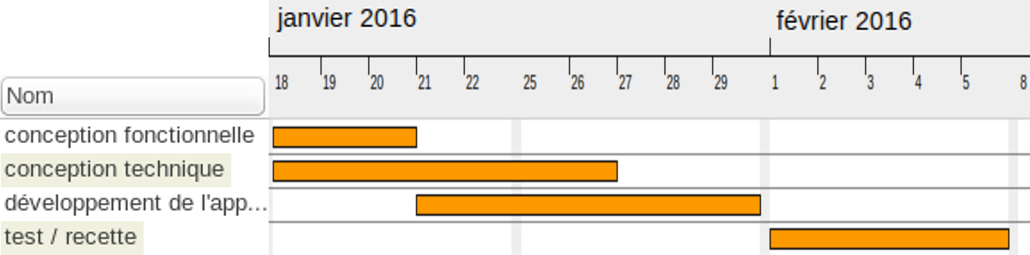
\includegraphics[width=15cm]{images/gantt.png}


\end{document}
